\documentclass[
	classe=1 STI2D,
	gray,
	surFeuille,
	headerTitle=Évaluation\space Chapitre\space 2
]{évaluation}

\usepackage{tcolorbox}
\usetikzlibrary{calc}

\title{Évaluation : Généralités sur les fonctions (sujet A)}
\author{}
\date{}

\begin{document}

\maketitle

\begin{tcolorbox}
	Cette évaluation est à rendre sur une feuille simple ou double.

	Ne pas oublier de mettre son nom et prénom sur sa copie, ainsi que le sujet (A).

	La calculatrice est \textbf{autorisée}.

	Toutes les réponses \textbf{devront être rédigées}, et les calculs \textbf{détaillés}.
\end{tcolorbox}

\begin{exercice}

	On a donné les graphes des fonctions $f$ et $g$ ci-dessous, définies sur l'intervalle $[-5; 5]$ :

	\begin{center}
		\begin{tikzpicture}[scale=0.7]
			\draw[very thin,gray] (-5.5,-4.5) grid (5.5,5.5);
			\draw[thick,\myArrow] (-5.5,0) -- (5.5,0);
			\draw[thick,\myArrow] (0,-4.5) -- (0,5.5);
			\foreach \x in {-5,-4,-3,-2,-1,1,2,...,5} {
					\draw (\x,0) -- ++(0,-0.2) node[below] {$\x$};
				}
			\foreach \x in {-4,-3,-2,-1,1,2,...,5} {
					\draw (0,\x) -- ++(-0.2,0) node[left] {$\x$};
				}
			\node[below left] at (0,0) {$0$};

			\draw[ultra thick,orange,domain=-5:-3,variable=\x] plot({\x},{41 + 19*\x + 2*\x*\x});
			\draw[ultra thick,orange,domain=-3:0,variable=\x] plot({\x},{-2 + 1/6*\x + 3*\x*\x + 5/6*\x*\x*\x});
			\draw[ultra thick,orange,domain=0:4,variable=\x] plot({\x},{-2 - 29/60*\x + 27/40*\x*\x - 11/120*\x*\x*\x});
			\draw[ultra thick,orange,domain=4:5,variable=\x] plot({\x},{7 - 3.5*\x + 0.5*\x*\x}) node[right] {$𝒞_f$};

			\draw[ultra thick,violet,domain=-5:5,variable=\x] plot({\x},{(-4*\x + 1/3*\x*\x*\x) / (65/12)}) node[right] {$𝒞_g$};
		\end{tikzpicture}
	\end{center}

	\begin{enumerate}
		\item Donner l'image par $f$ de $-4$ et $0$.
		\item Quelle est le sens de variation de $f$ sur $[1 ; 5]$ ?
		\item Calculer le taux de variation de $f$ entre $-2$ et $-2$.
		\item Donner l'image par $g$ de $-2$ et $5$.
		\item Donner, si ils existent, les antécédents par $g$ de $-1$, $1$ et $5$.
		\item Donner le tableau de variations de $g$.
	\end{enumerate}
\end{exercice}

\begin{exercice}
	Soit $f$ la fonction telle que $f(x) = 3x + 2$.

	\begin{enumerate}
		\item Résoudre l'équation $f(x) = 0$.
		\item En déduire le tableau de signes de $f$.
		\item Calculer le taux de variation de $f$ entre $-2$ et $2$.
		\item Calculer le taux de variation de $f$ entre $3$ et $6$.
		\item (BONUS) Montrer que quelque soient les nombres $a$ et $b$ choisis, le taux de variation de $f$ entre $a$ et $b$ est le même.
	\end{enumerate}
\end{exercice}

\begin{exercice}
	% 625€/tonne, il leur en faut 10 tonnes/mois
	Une entreprise achète 10 tonnes de papier chaque mois, pour $6\ 250$ €. \smallskip

	Étant elle-même producteur de carton, elle décide que produire le papier elle-même ne doit pas être si difficile. Elle achète donc à partir de maintenant le matériel nécessaire :

	\begin{itemize}
		\item La machine à fabriquer le papier, qui coûte initialement $120\ 000$ €.
		\item La pâte à papier, achetée $2\ 500$ € chaque mois.
		      % ~1000€/tonne
		\item L'eau nécessaire au traitement du papier, qui coûte $9\ 600$ € par an.
		      % 80€ pour 1 tonne de papier
	\end{itemize}

	\begin{enumerate}
		\item Au bout de combien de mois cette décision permettra à l'entreprise de réaliser des économies ?
		\item Avec sa machine, l'entreprise produit à présent $15$ tonnes de papier chaque mois. Elle décide donc de revendre les $5$ tonnes de surplus, pour $250$ € la tonne.

		      Avec cette nouvelle donnée, combien de mois lui faudra-t'elle pour réaliser des économies ?
	\end{enumerate}
\end{exercice}

\begin{exercice}
	On donne deux figures géométriques :

	\begin{center}
		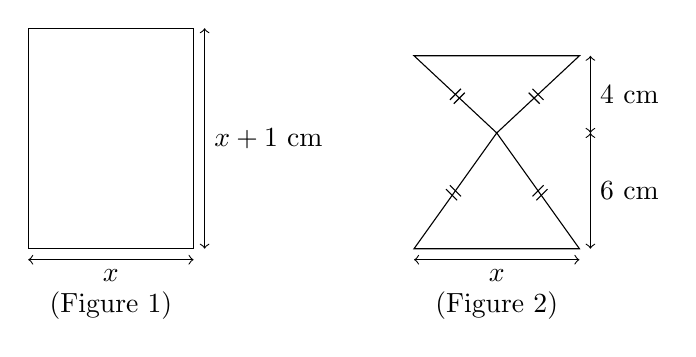
\begin{tikzpicture}[scale=0.7]
			\coordinate (Figure1) at (0,0);
			\coordinate (Figure2) at (7,0);

			\draw (Figure1) -- ++(3,0) -- ++(0,4) -- ++(-3,0) -- cycle;
			\node[below] at ($(Figure1) + (1.5,-0.6)$) {(Figure 1)};
			\draw[<->] (Figure1) ++(0,-0.2) -- node[below] {$x$} ++(3,0);
			\draw[<->] (Figure1) ++(3.2,0) -- node[right] {$x + 1$ cm} ++(0,4);

			\draw (Figure2) -- ++(3,0) -- ++(-1.5,2.1) -- cycle;
			\draw (Figure2) ++(1.5,2.1) -- ++(-1.5,1.4) -- ++(3,0) -- cycle;
			\node[below] at ($(Figure2) + (1.5,-0.6)$) {(Figure 2)};
			\draw[<->] (Figure2) ++(0,-0.2) -- node[below] {$x$} ++(3,0);
			\draw[<->] (Figure2) ++(3.2,0) -- node[right] {$6$ cm} ++(0,2.1);
			\draw[<->] (Figure2) ++(3.2,2.1) -- node[right] {$4$ cm} ++(0,1.4);
			\draw ($(Figure2) + (0.75,1.05)$) ++(-0.1,0.1) -- ++(0.2,-0.2) ++(-0.07,-0.07) -- ++(-0.2,0.2);
			\draw ($(Figure2) + (2.25,2.8)$) ++(-0.1,0.1) -- ++(0.2,-0.2) ++(-0.07,-0.07) -- ++(-0.2,0.2);
			\draw ($(Figure2) + (2.25,1.05)$) ++(0.1,0.1) -- ++(-0.2,-0.2) ++(0.07,-0.07) -- ++(0.2,0.2);
			\draw ($(Figure2) + (0.75,2.8)$) ++(0.1,0.1) -- ++(-0.2,-0.2) ++(0.07,-0.07) -- ++(0.2,0.2);
		\end{tikzpicture}
	\end{center}

	\begin{enumerate}
		\item Donner l'aire $𝒜₁(x)$ de la figure 1 en fonction de $x$ (en cm).
		\item Donner l'aire $𝒜₂(x)$ de la figure 2 en fonction de $x$ (en cm).
		\item Créer un repère du plan, dans lequel :
		      \begin{itemize}
			      \item En abscisse, un centimètre représente une longueur de 1 cm.
			      \item En ordonnée, un centimètre représente une aire de 10 cm².
		      \end{itemize}
		      Représenter graphiquement les fonctions $𝒜₁$ et $𝒜₂$ dans ce repère, pour $x$ entre $0$ et $10$ variant de centimètre en centimètre.
		\item Pour quelle valeur de $x$ les deux aires sont-elles égales ? Quelle est alors l'aire obtenue pour chaque figure ?
	\end{enumerate}
\end{exercice}

\end{document}